\chapter{Motivations}

Cancer is considered to be the second biggest killer after cardiovascular diseases: there were an estimated 14.1 million cancer cases around the world in 2012, of these 7.4 million cases were in men and 6.7 million in women. This number is expected to increase to 24 million by 2035 \cite{Ferlay2012}.

Although surgery remains the most diffuse and successful treatment, radiotherapy is an important and effective option used for curative and palliative management of malignant tumors.
In approximately the $50\%$ of clinical cases, radiation therapy is a part of the initial treatment and it is usually conducted by means of high-energy X-rays \cite{Durante2010}.

Results of radiotherapy are improved when a high dose of radiation with high biological effectiveness is delivered to the tumour with the least possible dose to the surrounding tissues, especially in the case of critical organs \cite{Linz2011}.
In order to increase the conformity of the dose delivered to the tumour, diverse technologies have been considered and used.
Traditional forms of radiotherapy, X-ray tubes (energy $\sim$ 100 keV) or radioactive isotopes, have been replaced by linear accelerator delivering ($\sim$ 10 MeV) from different directions (e.g. Intensity Modulated Radio Therapy).
Although being widely used as a standard in radiation therapy, the effectiveness of conventional electromagnetic radiation is limited by the intrinsic characteristics of interaction with matter.
With respect to this, the scientific community is focusing its attention towards possible improvements of ion beam therapy \cite{Amaldi2011}.
In particular two aspects disfavours the usability of electromagnetic radiation with respect to ion for tumour targeting: the depth dose profile, which does not allow for an optimal dose deposition to the tumour sparing vital organs,
and the inferior biological effectiveness, which is the limiting factor in case of radio resistant tumours.
Heavier charged particles, like protons and ions (He-Ca) have the potentiality to overcome the limits of conventional therapy. 
As explained in the next section, ion beam therapy is more effective for targeting deep lying  or inoperable tumours.
The issues connected to range uncertainties require the development of an effective imaging technique for beam monitoring. 
Since this thesis is focused on the operational parameters of one of these techniques, Time-Of-Flight Positron Emission Tomography, a brief introduction of ion beam techniques and in-vivo monitoring is given in this chapter.

\begin{figure}
\centering
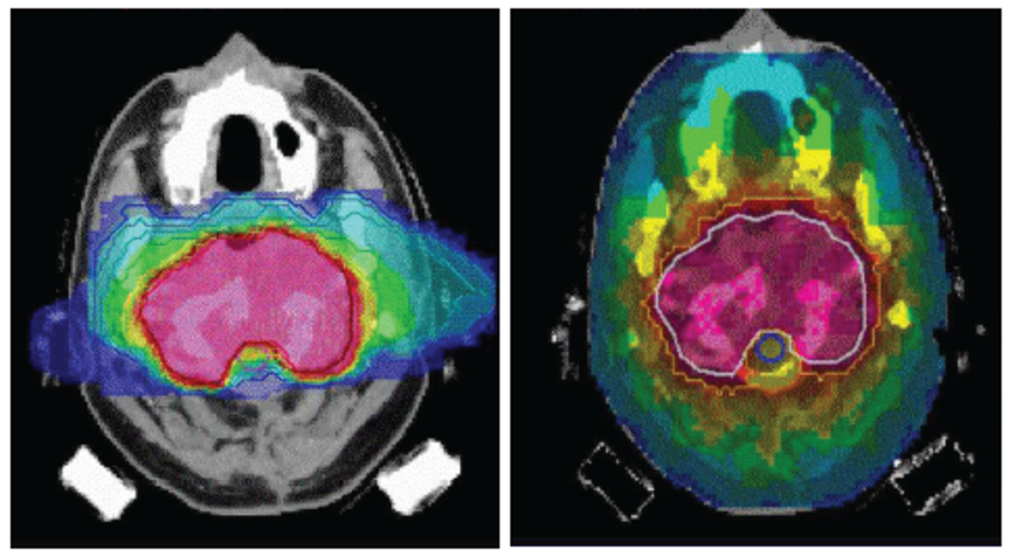
\includegraphics[width=12cm]{Pictures/Chapter_1/treat_conf2.pdf}
\caption[X-ray and proton irradiation]{Comparison of treatment plans for a large target volume in the base of the skull. Plan for carbon ions (left) and IMRT (right) \cite{Durante2010}.}
\label{fig:irradiation}
\end{figure}

\section{Particle therapy}
\subsection{Ion beam therapy}

The first proposition of ion beam therapy was presented in 1946 by R. Wilson \cite{Wilson1946}. The original idea was to exploit the physical properties of ion interaction in matter to improve the precision in radiotherapy treatments.  
Making use of the so called Bragg peak, that is using the fact that protons and ions in general deposit a maximum of energy at the end of their trajectory, the treatment could save the surrounding tissue from radiation overdose.

\begin{figure}
\centering
\begin{subfigure}
  {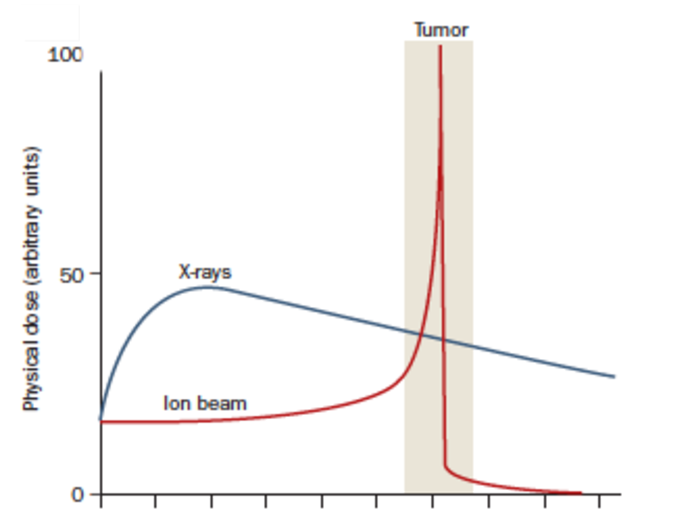
\includegraphics[width=6cm]{Pictures/Chapter_1/profile.pdf}}
\end{subfigure}
\begin{subfigure}
  {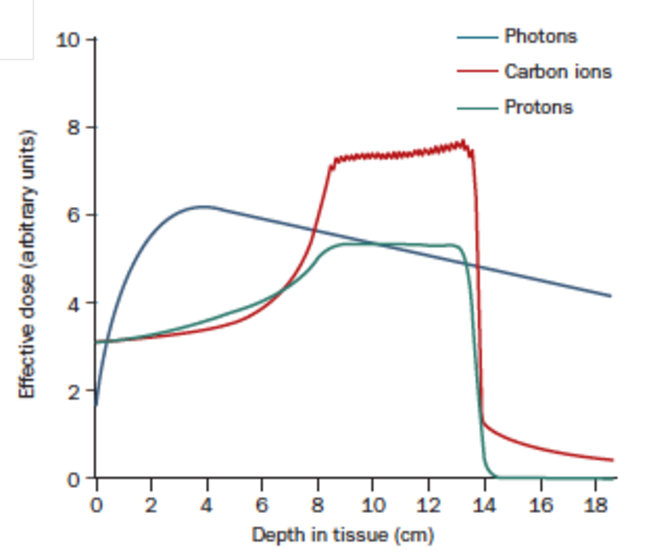
\includegraphics[width=6cm]{Pictures/Chapter_1/SOBP.pdf}}
\end{subfigure}
\caption[Depth dose comparison]{Comparison of the depth–dose relationships for X-rays and high-energy charged particles. In treatment of large tumors, the Bragg peak must be broadened by use of overlapping beams with different energies \cite{Durante2010}.}
\label{fig:test}
\end{figure}

The dose deposited by photons, considered as the gold standard for tumour treatment, is maximum close to the beginning of the trajectory in the body and is characterized by an exponential decrease. As a consequence, an undesired radiation dose is delivered to healthy tissues around the targeted tumour.

The recent therapeutic interest of ions in the field of radiotherapy relies mainly on their high relative biological effectiveness.
LET (linear energy transfer) has long been viewed as the main parameter to discern the biological effect of different kinds of radiation. It is a measure for the energy deposited by a charged particle traveling through matter. LET is closely related to stopping power and is not a constant value, since it changes along the particle's path (es 10 KeV/$\mu$m for photons, 100 KeV/$\mu$m for protons, 1000 KeV/$\mu$m for ions).
When considering ions of different atomic number LET becomes a limited parameter to evaluate the biological effect. 

In this sense the relative biological effectiveness (RBE) is considered the most accurate quantity, since it is defined as the biological effect of one type of ionizing radiation relative to another, given the same amount of absorbed energy. As the charge of the incident ions increases, so does the probability of severe DNA damage. An elevate RBE in the Bragg peak region has clearly been demonstrated for ions heavier than Helium  \cite{Linz2011}.
As a consequence they prove to be more effective for targeting radio resistant or inoperable tumours.

%rbe
\begin{figure}  
\centering
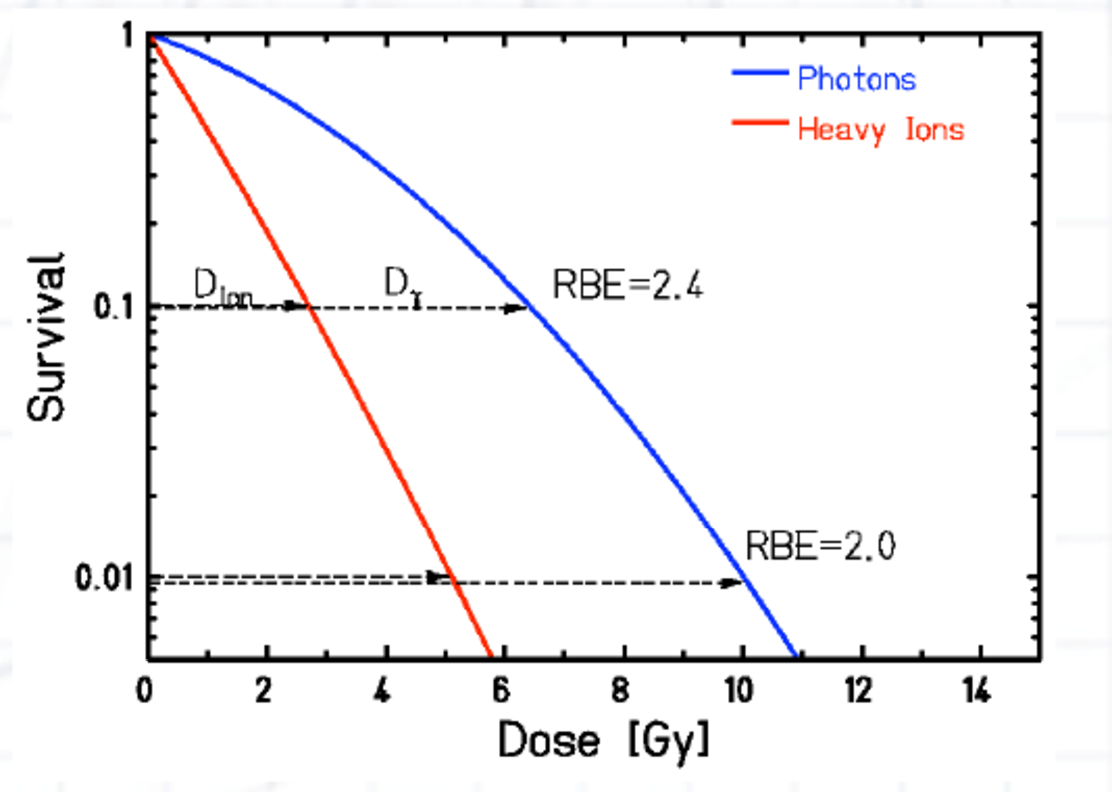
\includegraphics[width=8cm]{Pictures/Chapter_1/rbe.pdf}
\caption[RBE comparison]{Comparative plot of RBE for photons and heavy ions.}
\label{fig:rbe}
\end{figure}

\subsection{Beam delivery}

Ion beams are delivered by either cyclotrons or synchrotrons. In the first case the beam has a fixed energy which is tuned by means of degraders in order to deliver the correct dose profile. In the case of synchrotron the beam is delivered in spills and the energy is varied between spills. In the case of Carbon only synchrotrons can be used.
To deliver the dose to the planned target volume (PTV) different energies are superimposed in order to obtain the so-called spread-out Bragg peak (SOBP). The beam is usually delivered in a passive beam shaping setup or a scanning system. 

Different sources of error can worsen the dose delivery profile, such as patient mis positioning and evolution of the tumour/morphology of the patient. In addition the complex physics of ion interaction leads to  imprecisions in the treatment plannings, due to fragmentation of the incident beam and range uncertainties.

Usually treatment planning systems cope with these problems by irradiating a volume larger than the tumour itself, called planning target volume (PTV) which contains the clinical target volume (CTV). Complex compensating systems, including x-ray imaging techniques and patient positioning systems, allow to reduce errors in the dose profiles delivered. 
Treatment plannings of ion therapy rely for example on accurate values of particle range in tissue obtained from Hounsfield unit of computed tomograms, leading to uncertainties of $1-3\%$ in range calculations \cite{Enghardt2004}.

The dose delivered by a ion beam system is much more sensitive to these deviations than the one delivered by a photon beam. Due to the high biological effectiveness of ion beams, wrong ranges could lead to dramatic under dosage to the tumour or over dosage to organ at risk surrounding.
As a consequence a three-dimensional non invasive imaging technique for ion beam therapy monitoring is required. Since ions, unlike photons, are stopped completely in the patient volume, technology like portal imaging are not suitable. The attention of the community is thus focused on positron emission tomography (PET), which relies on the peculiar characteristics of $\beta ^{+}$ decay.

%prblemi di deliver
\begin{figure} 
\centering 
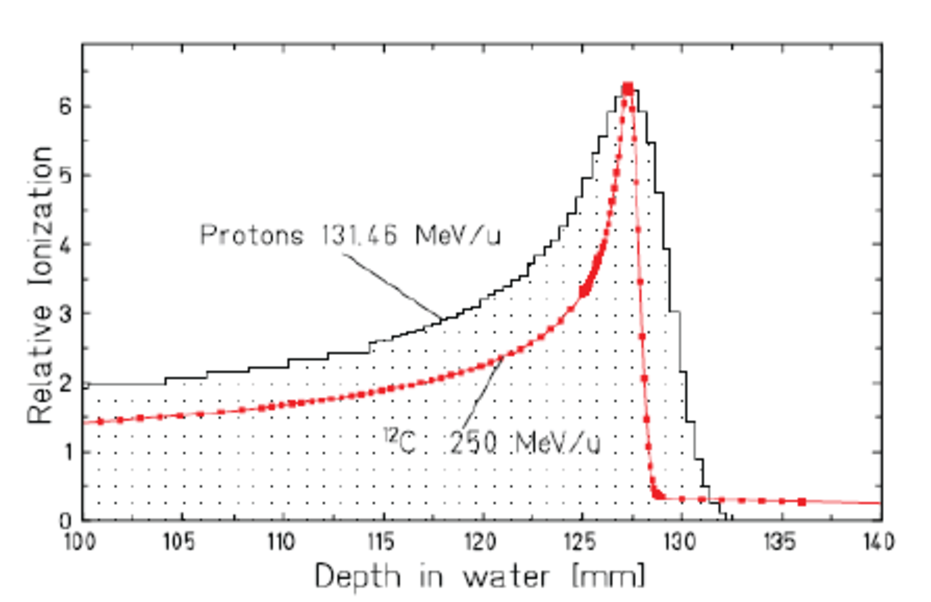
\includegraphics[width=8cm]{Pictures/Chapter_1/range_scatter.pdf}
\caption[Peak spread for Carbon]{Bragg curves of proton and C-ions having the same mean range (water phantom and ionization chamber) \cite{Schardt2007}.}
\label{fig:spread}
\end{figure}

\subsection{Monitoring of the beam}

Several attempts have already been undertaken to systematically assess the benefit of the PET method for beam monitoring, the principal one being the set up installed at the experimental carbon ion therapy unit at the Gesellschaft fur Schwerionenfroschung Darmstadt (GSI) \cite{Parodi2004}.
Two alternatives can be considered: the use of positron radioactive ions as projectiles for dose delivery or the detection of $\beta ^{+}$ activity given by nuclei fragmentation.
As an example of the first approach it is interesting to consider the effort made at the Heavy Ion Accelerator in Chiba (Japan), where radioactive beams of $^{11}C - ^{10}C$ ions deliver an activity of $10^{3} - 10^{5}$ $Bq$ $Gy^{-1}$ cm$^{-3}$ within the irradiated volume.
Due to the low production rate of secondary radioactive ions, this approach has been only partially successful.

Another possibility is to make use of the $\beta ^{+}$ activation given by the fragmentation of stable ions interacting with the tissue.
The radioactivity is a direct product of the irradiation and, although the activity density is rather low (around 600 $Bq$ $Gy^{-1}$ cm$^{-3}$ for protons), this method provides a rather cheaper and feasible solution \cite{Enghardt2004}.
The activity slides very fast under a reasonable threshold for detectability and the most effective solution is an in-beam scanner.
In-beam PET is currently the main method implemented clinically for in situ monitoring of charged hadron radiotherapy \cite{Crespo2007}.

% attivita irraggiamento!!!!!

%\begin{figure}  
%\includegraphics[width=\textwidth]{Pictures/Chapter_1/conformal_x_rays}
%\caption[Short figure name.]{Schematic view of depth-dose distributions of photons and ions. (a) photon
%field, (b) spread-out ion beam, (c) depth–dose profiles along the central beam axis \cite{Linz2011}.}
%\label{fig:myInlineFigure}}
%\end{figure}

\section{Positron Emission Tomography}
\subsection{Principles}
Positron Emission Tomography (PET) has been introduced as a nuclear medicine imaging technique which measures the distribution of a positron-emitting radionuclide (tracer), which is injected into the body on a biologically active molecule. In the case of in-beam PET the activity is present in the body of the patient due to the activation induced by proton interaction.

After the injection, or during the dose delivery, the subject of a PET study is placed within the field of view (FOV) of a number of detectors capable of registering incident $\gamma$ rays. The radionuclide in the radio tracer decays and the resulting positrons subsequently annihilate with electrons after travelling a short distance ($\sim$ 1 mm) within the body.

Each annihilation produces two $511$ keV photons travelling in opposite directions and these photons may be interact with detectors surrounding the subject. The detector electronics are linked so that two detection events unambiguously occurring within a certain time window may be called coincident and thus be determined to have come from the same annihilation. These events can be stored in arrays corresponding to projections through the patient and reconstructed using standard tomographic techniques. The resulting images show the tracer distribution throughout the body of the subject. The scheme of a PET scanner is shown in figure  \ref{fig:PET}.

As already mentioned, positron emission tomography relies on the $\beta ^{+}$ decay of a radionuclide.
% pet schema
\begin{figure}
\centering  
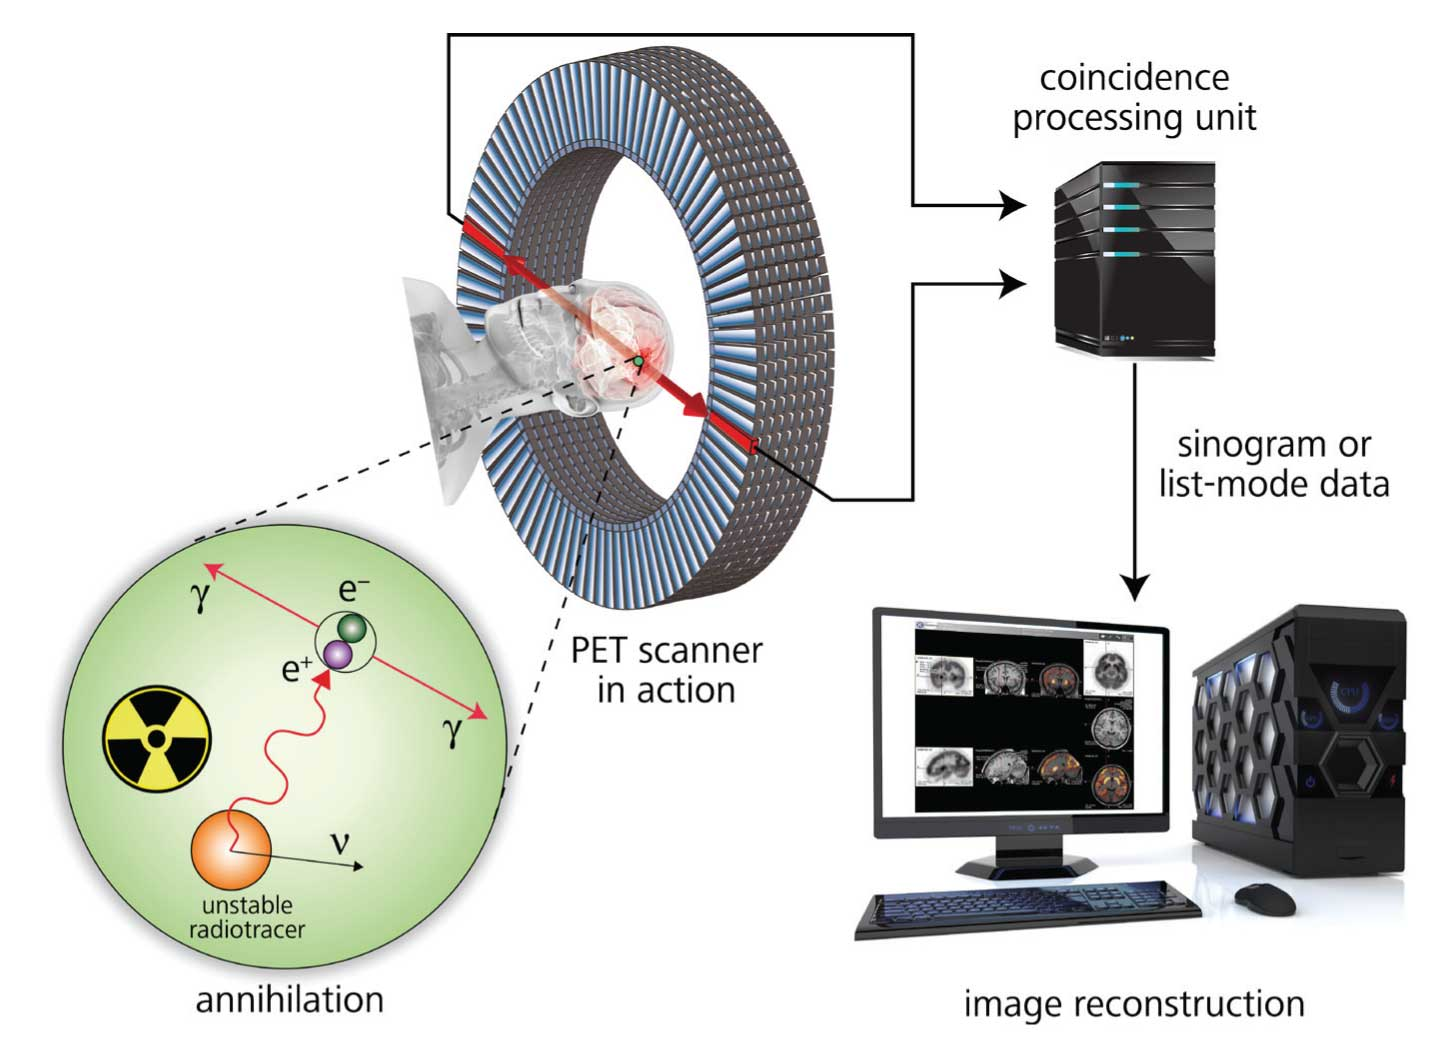
\includegraphics[width=8cm]{Pictures/Chapter_1/PET_scheme}
\caption[PET scanner]{Schematic view of PET scanner.}
\label{fig:PET}
\end{figure}
The nucleus of the radionuclide can convert a proton into a neutron 
\begin{displaymath}
p\rightarrow n + e^{+} + \nu _{e}
\end{displaymath}
As positrons travel through human tissue, they give up their kinetic energy principally by Coulomb interactions with electrons. As the rest mass of the positron is the same as that of the electron, the positrons may undergo large deviations in direction with each Coulomb interaction, and they follow a tortuous path through the tissue as they give up their kinetic energy.

When the positrons reach thermal energies, they start to interact with electrons either by annihilation, which produces two $511$ keV anti-parallel photons, or by the formation of a hydrogen-like orbiting couple called positronium. In its ground-state, positronium has two forms: ortho-positronium, where the spins of the electron and positron are parallel, and para-positronium, where the spins are anti-parallel. Para-positronium again decays by self-annihilation, generating two anti-parallel $511$ keV photons. Ortho-positronium self-annihilates by the emission of three photons. Both forms are susceptible to the pick-off process, where the positron annihilates with another electron. Free annihilation and the pick-off process are responsible for over $80\%$ of the decay events.

\subsection{Image reconstruction}

After all corrections have been applied to the data acquired, the number of counts assigned to a LOR joining a pair of crystals is proportional to a line integral of the activity along that LOR. Parallel sets of such line integrals are known as projections.
These projections are usually graphically represented as a sinogram, which collects the intensity valuesof the voxels in the coordinate system of variables $\phi$ and s, as shown in figure \ref{fig:reco}.

For image reconstruction, the most commonly used algorithms are the analytical method called filtered back projection and iterative reconstruction schemes.
% sinogram reco
\begin{figure} 
\centering 
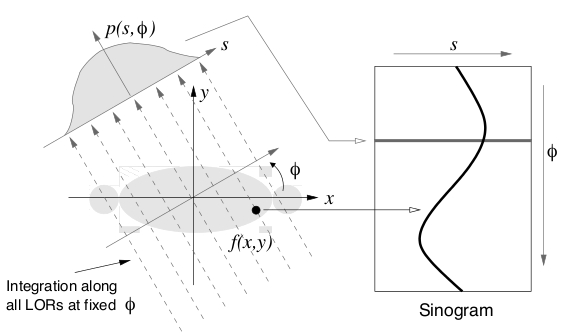
\includegraphics[width=8cm]{Pictures/Chapter_1/proj_sin.jpg}
\caption[Image reconstruction in PET]{Extraction of a sinogram from a 2D acquisition.}
\label{fig:reco}
\end{figure}
In particular iterative methods are often preferred over analytical approaches because they can account more effectively for the noise structure and can use a more realistic model of the system. Moreover advances in computation speed and faster algorithms allowed iterative methods to receive growing clinical acceptance.
An iterative method has five basic components.
\begin{itemize}
\item A model for the image, that is a discretization of the image domain into pixels (2-D) or voxels (3-D) or other exotic models.
\item A system model that relates the image to the data. A system model M is characterized by elements $M_{ij}$ related to the image system that represent the probability that an emission from voxel j is detected in projection i
\item A model for the data which describes the statistical relation between the value obtained and the value expected
\item A governing principle that defines the parameters of a "best" image, often expressed as a cost function (e.g. Maximum likelihood)
\item An algorithm that optimizes the cost function.
\end{itemize}

This last issue has been implemented in several ways, ranging from gradient-based algorithms to the commonly used Expectation Maximization (EM) algorithm and its variations (OSEM).

\subsection{Sources of noise and sensitivity}
In a PET scanner, each detector generates a timed pulse when it registers an incident photon. These pulses are then combined in coincidence circuitry, and if the pulses fall within a short time-window, they are deemed to be coincident.
A coincidence event is assigned to a line of response (LOR) joining the two relevant detectors. In this way, positional information is gained from the detected radiation without the need of a physical collimator. This is known as electronic collimation.
When a physical collimator is used, directional information is gained by preventing photons which are not normal or nearly normal to the collimator face from falling on the detector. In electronic collimation, these photons may be detected and used as signal.
Coincidence events in PET fall into four categories: true, scattered, random and multiple, as shown in figure \ref{fig:coinc}. 

True coincidences occur when both photons from an annihilation event are detected by detectors in coincidence, neither photon undergoes any form of interaction prior to detection, and no other event is detected within the coincidence time-window.

% coincidenze
\begin{figure}  
\centering
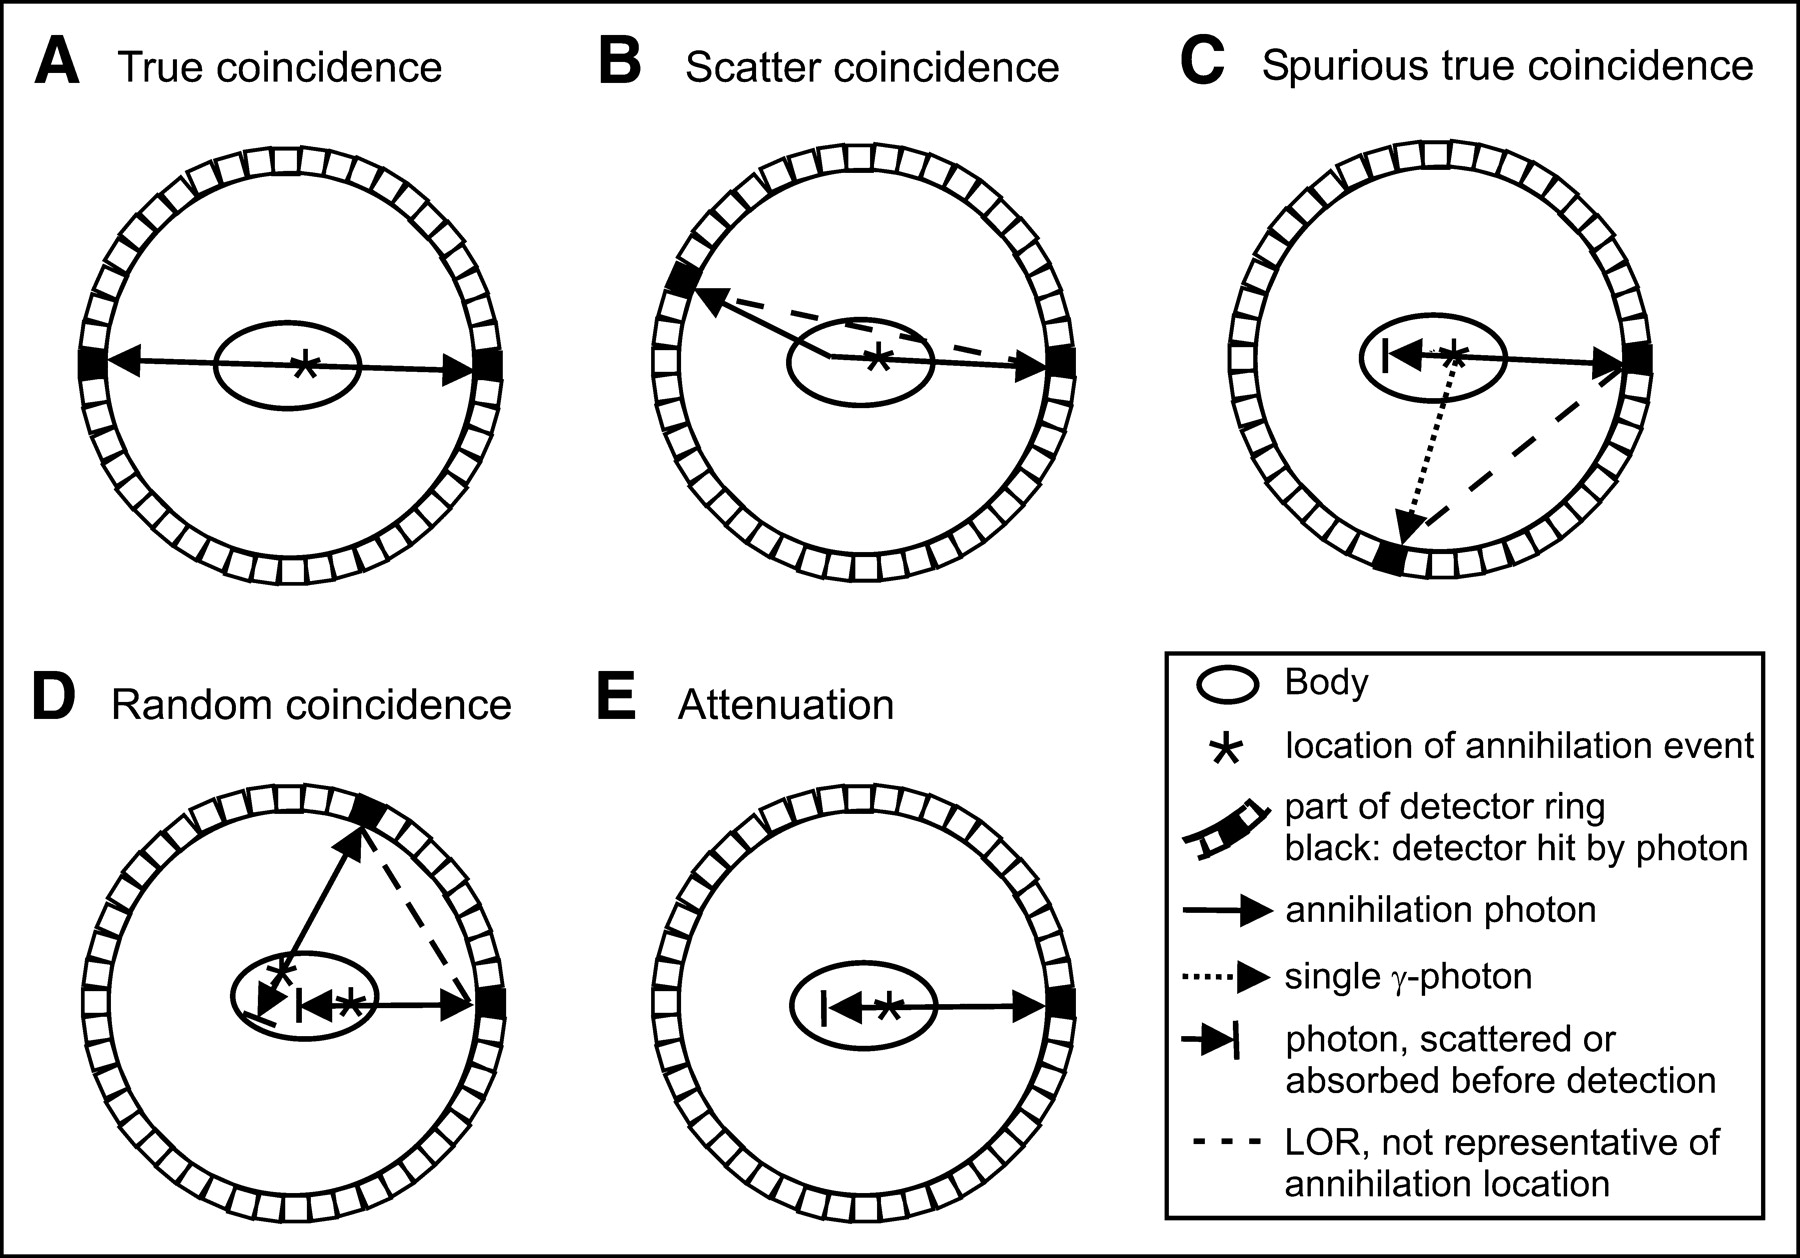
\includegraphics[width=8cm]{Pictures/Chapter_1/coinci_PET}
\caption[Coincidencies in PET exam]{Phenomelogy of PET examination. The cases b, c, d lead to loss of resolution.}
\label{fig:coinc}
\end{figure}

A scattered coincidence is one in which at least one of the detected photons has undergone at least one Compton scattering event prior to detection. Since the direction of the photon is changed during the Compton scattering process, it is highly likely that the resulting coincidence event will be assigned to a wrong LOR. Scattered coincidences add background to the true coincidence distribution which changes slowly with position, decreasing contrast and causing the isotope concentrations to be overestimated. They also add statistical noise to the signal. The number of scattered events detected depends on the volume and attenuation characteristics of the object being imaged, and on the geometry of the PET scanner.

Random coincidences occur when two photons not arising from the same annihilation event are incident on the detectors within the coincidence time window of the system. The number of random coincidences in a given LOR is closely linked to the rate of single events measured by the detectors joined by that LOR and the rate of random coincidences increase roughly with the square of the activity in the FOV. As with scattered events, the number of random coincidences detected also depends on the volume and attenuation characteristics of the object being imaged, and on the geometry of the scanner. The distribution of random coincidences is fairly uniform across the FOV, and will cause isotope concentrations to be overestimated if not corrected for. Random coincidences also add statistical noise to the data.
\newpage
\subsection{Time-Of-Flight PET}

It has been shown that in-beam PET could not provide definitive information to the oncologist when medium to large tumors are involved \cite{Fiedler2006}. This is due to the operative parameters of scanners available on the market, with relatively slow scintillators and tomographs covering small solid angles. A decisive improvement could be given by time-of-flight PET (TOF-PET).

Recent developments in scintillator technology and read out electronics allow to build detectors able to detect the time difference between the moment of detection of the opposed $\gamma$ rays in coincidence. 
%tof pet
\begin{figure}
\centering  
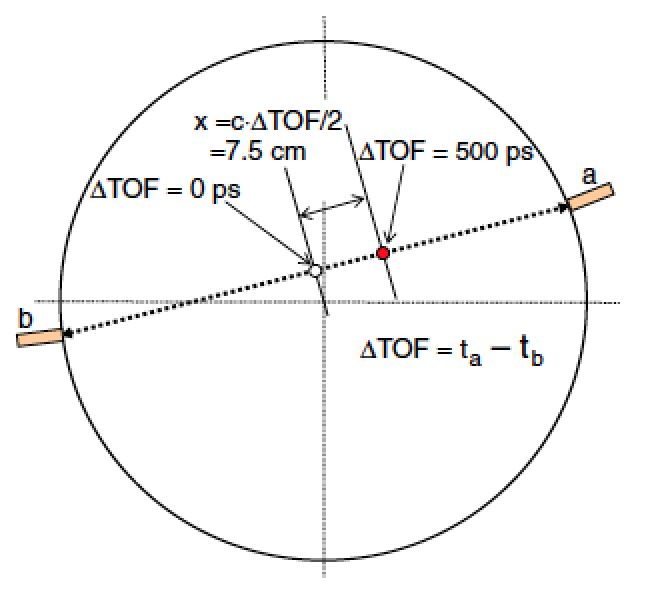
\includegraphics[width=6cm]{Pictures/Chapter_1/TOF}
\caption[TOF-PET schematics]{Example of time of flight information usage in PET examination.}
\label{fig:TOF}
\end{figure}
If we define a LOR between two detectors A and B, the distance between the center of the LOR and the annihilation point is given by
\begin{equation}
x = (t_{b}-t_{a} ) \cdot c/2
\end{equation}
where c is the speed of light. This situation is depicted in figure \ref{fig:TOF}.
Thus the spatial resolution is proportional to the coincidence time resolution (CTR) of the system.
Scanners available on the market today could deliver a 600 pico seconds time resolution, that translates to a positional uncertainty of 9 cm (FWHM) on the LOR.
The quality of the tomographic image largely benefits from the timing information of a TOF-PET scanner, since it reduces considerably  the contribution of Compton scattered photons and from photons from outside the field-of-view (FOV).
As a consequence the background from scattered and random coincidence is largely suppressed. 
The signal to noise ration (SNR) is thus dramatically improved, as we can write \cite{Karp2008}:
\begin{equation}
SNR \propto \frac{1}{\sqrt{n}}\left[ \frac{T^{2}}{T^{2} + S + R} \right]^{1/2}
\end{equation}
where where T representes the total trues, R thee random coincidences, S the scattered coincidence and n is the number of image elements contributing to a projection of the sinogram.
In the case of in-beam PET this is relevant, since it has been shown \cite{Fiedler2006} that during particle irradiation a considerable amount of activity is transported outside the FOV by metabolic processes. Moreover a high backround signal is typical of carbon ion beams \cite{Enghardt2004}. 
A useful and pratical estimation of the gain in signal to noise can be formalized as follows
\begin{displaymath}
G = \frac{SNR_{TOF}}{SNR_{non_{TOF}}} = \sqrt{\frac{2\cdot D}{c \cdot CTR}}
\end{displaymath}
where D is the diameter of the volume under examination, c is the speed of light and CTR is the coincidence time resolution. Thus a CTR of 100 ps FWHM translates into a 1.5 cm resolution on the position and a SNR gain of 5 (corresponing to a sensitivity gain of about a factor 25) compared to non TOF systems.

% quanto guadagni con tofpet
\begin{figure}  
\centering
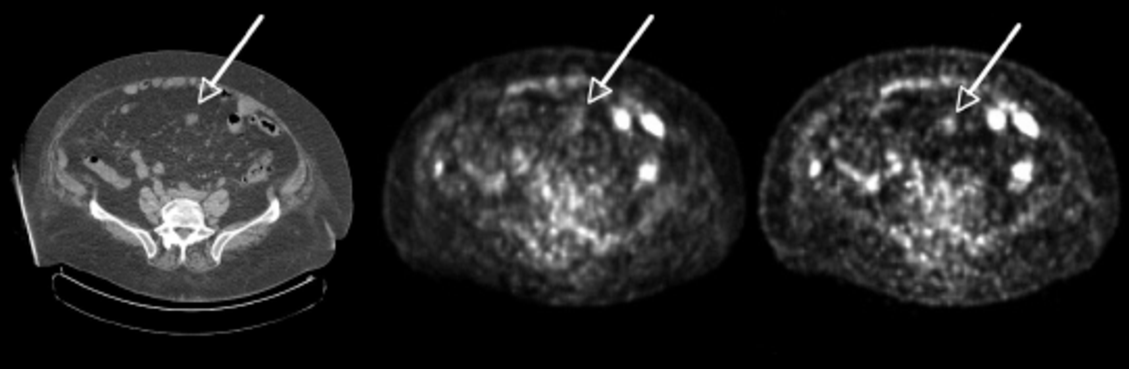
\includegraphics[width=14cm]{Pictures/Chapter_1/tof_gain.pdf}
\caption[Improvement of TOF-PET]{Representative transverse sections: low dose CT (left), non-TOF ML-EM (middle), and TOF ML-EM (right). The patient with colon cancer (119 kg, BMI = 46.5) shows a lesion in the abdomen seen in CT much more clearly in the TOF image than in the non-TOF image \cite{Karp2008}.}
\label{fig:tofgain}
\end{figure}

\section{Outline of the thesis}

\subsection{From high energy physics to medical applications}
The work outlined in these pages have been sponsored by \textit{The European training network in digital medical imaging for radiotherapy} (ENTERVISION) at the \textit{European Center of Nuclear Research} (CERN). ENTERVISION was established in February 2011 in response to the critical need for reinforcing research in online 3D digital imaging in order to deliver some of the key elements and building blocks for realizing the vision for early detection and more precise treatment of tumours.
The present work was hosted by CERN, the European Organisation of Nuclear Research, based in Geneva, Switzerland. 
CERN was established by a formal act in Paris, on 1st of July 1954, as an organisation that \textit{shall provide for collaboration among European States in nuclear research of a pure scientific and fundamental character, and in research essentially related thereto}.
Thourought its history, CERN provided experimental and theoretical tools to study and understand the fundamental forces governing our universe, in a continous effort to improve our understanding of elementary  physics. 

The ECAL detector at the CMS exeriment at the LHC was build with the fundamental contribution of the collaboration hosting this thesis: the Crystal Clear Collaboration. It was founded in 1990 as an international academic network of laboratories and industrial partners for the development of scintillating crystal detectors as well as their applications. It comprises experts in crystallography and solid state physics as well as in radiation detection and instrumentation. 
Its first goal was the development of a radiation-hard crystal for the ECAL detector, leading to the development of PbWO4 (PWO) as the material selected for CMS calorimeter. More recently the group has been focusing on the study of new materials for hadronic and electromagnetic calorimeters for future particle accelerators.
In parallel, the collaboration engaged in a effort of technology transfer to other domains exploiting the expertise developed in scintillating detectors. It is quite natural to focus the attention to medical physics, with particular respect to nuclear medicine since the requirements for detectors used in medical physics and detectors for high energy experiments are similar.

% high energy requirements
%\begin{figure}  
%\includegraphics[width=\textwidth]{Pictures/Chapter_1/conformal_x_rays}
%\caption[Short figure name.]{Schematic view of depth-dose %distributions of photons and ions. (a) photon
%field, (b) spread-out ion beam, (c) depth–dose profiles along the %central beam axis \cite{Linz2011}.}
%\label{fig:myInlineFigure}}
%\end{figure}

\subsection{Study of time profiles}

This thesis is devoted to the full characterization of the parameters that influence time resolution in a scintillator/photodetector setup, with particular attention focused on the impact of time profiles of heavy scintillators on the performance.

The first part of the presented work has the objective of describing the fundamental model that governs light production and collection in a PET-like setup.
In chapter 2 and 3 a brief introduction regarding heavy scntillator crystals and photodetectors is given.

With the objective of defining the operational parameters of our equipment, in chapter 3 a model based on multi-exponential time profiles has been implemented on an existing framework, widening the scope of usage by evaluating the role of Cerenkov photons produced by low energy radiation.

Moreover in order to properly characterized the operational parameters of a scintillator setup, a comparative analysis of ray tracing softwares has been conducted in chapter 5, namely the two packages SLitrani and Geant4. The latter has been chosen to build the simulation framework that allowed to disentangle the various source of resolution degradation.

Finally the work focused on the measurements and evaluation of rise time. Non zero rise time in scintillating systems is given by the different processes characterizing energy deposition inside a crystalline lattice, with utmost relevance of the latest stage of electron hole thermalization. The time scale of this phenomenon is $\sim$ 100 ps and until now has proven to be difficult to estimate due to the intrinsic limitations of detection setups.
Thus a time resolved study of different species of crystals is proposed in the final part of this work.
In chapter 6 the methodology followed is presented, from an experimental point of view and defining the main challenges of data analysis.
Finally the last two chapters present the time resolved study, with excitation energy varied from the 36 eV of a VUV femto second source to the 511 KeV of a $\gamma$ source. 


%\afterpage{\clearpage}


